\chapter{Methods for inferring pairwise co-location}

With the data extracted and formatted in suitable manner, as described in the previous chapter, we move on to the main part of the thesis. Given a set of consecutive Bluetooth RSSI measurements, \textit{can we infer co-location?}; and if yes, what is the best way of doing it? 

One way of answering these questions is to simply set a threshold, and split the dataset into two parts: the ones that are above the threshold indicate co-location, while the other do not. That is exactly what \textit{Sekara,Lehmann} did in \cite{vedran}, with convincing results. They set the threshold to \textit{ -80 dBm}. 

On a similar note, we average our two types of data, the ones tagged \textit{yes} and \textit{no}, and we obtain an average of \textit{-64 dBm} for the ones tagged \textit{yes} and an average of {-82 dBm} for the ones tagged \textit{no}. From this result, one can easily see the similarity between the threshold in \textit{Sekara,Lehmann}'s work and the values obtained through this thesis's data, further indicating the validity of this result. 

The above method can successfully be used under any type of measurements. However, it does not take advantage of the additional information that our method of data gathering has provided, such as temporal information, or the significance of continuous measurements. Below we propose three methods of inferring pairwise co-location in the form of three machine learning algorithms. For each one we will provide a theoretical overview and implementation details. The chapter will end with a comparison between the three algorithms where results, ease of use and performance will be taken into consideration. 

While the parameters and the inputs used differ from one algorithm to another, one thing that remains constant across all of them is the testing methodology, described in the following section.

\section{Testing methodology}

In order to test the accuracy of the algorithms, we use cross-validation, a well recognized method for computing accuracy estimations \cite{kohavi1995study}. The technique is used here for obtaining an accuracy score for each algorithm and its variations, so that a comparison can be made at the end. Broadly speaking, cross-validation refers to the techniques used to partition the main dataset into two sets: a \textit{training} set, used in the initial phase for training the algorithms, and a \textit{testing} set, used for validating the algorithm with \textit{unseen before} data, after the training has finished. Two methods were used: k-fold validation, with $k = 10$ \cite{kohavi1995study}, and repeated random sub-sampling validation, with a $80-20$ proportion \cite{segaran}. 

\begin{itemize}
  \item K-fold validation is done by partitioning the data in k sets. One set is used for testing, while the the other $k-1$ are used for training. The processed is repeated $k$ times, once for each partition. The end result is the average over all $k$ results obtained. 
  \item For random sub-sampling validation, the dataset is partitioned into two sets. The entries are randomly assigned to one of the sets based on the proportion established at the beginning. For this type of validation, the test has been repeated 100 times, and the results averaged.   
\end{itemize}

During the execution of the tests, both k-fold validation and repeated random sub-sampling validation output extremely similar results, most of the time the results having a less than $0.5\%$ difference between them. For this reason, when presenting an algorithm score, that score will be the average of the two methods. 


\section{Neural Networks}

A first approach aims to use artificial neural networks (ANN) in order to infer co-location. 

\subsection{Theoretical overview}

The introduction of backpropagation by Rumelhart et al. \cite{rumelhart} paved the way for the development of the modern artificial neural network. In their current form, ANNs can be described as a network of processing units, called \textit{neurons}, or \textit{artificial neurons}. 

The general layout of an ANN can be seen in Fig. \ref{pic:ann}. It consists of an input layer, one or more hidden layers and an output layer. The number of \textit{neurons} on the input layer is equal with the number of features that represent the object we need to classify. The number of \textit{neurons} in the output layer usually equals the number of classes the objects need to be classified in. The number of hidden layers, and the number of \textit{neurons} in those layers varies greatly from problem to problem, and will be discussed in the next section, which tackles the implementation details. 

\begin{figure}[h]
	\begin{center}
		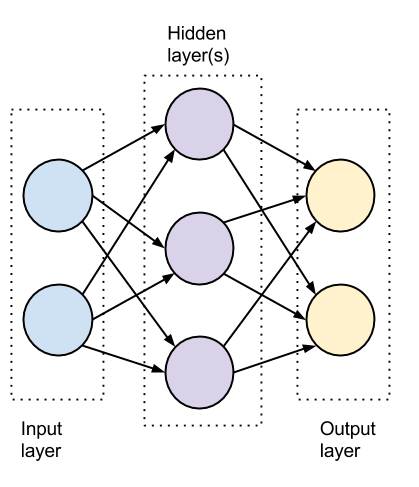
\includegraphics[scale=0.6]{figures/ANN.png}
	\end{center}
	
	\caption{General structure of an ANN.}
	\label{pic:ann}

\end{figure} 

A neural network has two main components

\subsection{Implementation}


\section{Regressive data}

\subsection{Theoretical overview}

\subsection{Implementation}


\section{Naive Bayes}

\subsection{Theoretical overview}

\subsection{Implementation}

\section {Comparison between the algorithms}